\documentclass[a4paper, openany]{memoir}

\usepackage[utf8]{inputenc}
\usepackage[T1]{fontenc} 
\usepackage[english]{babel}

\usepackage{fancyhdr}
\usepackage{float}

\usepackage{amsmath}
\usepackage{amsthm}
\usepackage{amssymb}
\usepackage{enumitem}
\usepackage{multicol}
\usepackage[bookmarksopen=true,bookmarksopenlevel=2]{hyperref}
\usepackage{tikz}
\usepackage{listings}
\usepackage{xcolor}
\usepackage{indentfirst}
\usepackage{caption}
\usepackage{subcaption}

\pagestyle{fancy}
\fancyhf{}
\fancyhead[LE]{\leftmark}
\fancyhead[RO]{\rightmark}
\fancyhead[RE, LO]{Algorithmics II}
\fancyfoot[LE, RO]{\thepage}
\fancyfoot[RE, LO]{Pete Gautam}

\usetikzlibrary{positioning, automata, arrows}

\definecolor{codegreen}{rgb}{0,0.6,0}
\definecolor{codegray}{rgb}{0.5,0.5,0.5}
\definecolor{codepurple}{rgb}{0.58,0,0.82}
\definecolor{backcolour}{rgb}{0.95,0.95,0.92}

\lstdefinestyle{thestyle}{
    backgroundcolor=\color{backcolour},
    basicstyle=\ttfamily\footnotesize,
    keywordstyle=\color{red!80}\bfseries,
    ndkeywordstyle=\color{blue!80}\bfseries,
    identifierstyle=\color{black},
    commentstyle=\color{codegreen},
    stringstyle=\color{codepurple},
    breakatwhitespace=false,
    breaklines=true,
    captionpos=b,
    keepspaces=true,
    numberstyle=\tiny\color{codegray},
    numbers=left,
    numbersep=2pt,
    showspaces=false,
    showstringspaces=false,
    showtabs=false,          
    tabsize=2
}

\lstdefinelanguage{pseudocode}{ 
    keywords={new, return, this, null, if, in, while, else, for, get, set, class, and, or, not, range},
    ndkeywords={int, char, bool, void, double, true, false, Line, LineSegment, Point, Rectangle, List, Map},
    sensitive=true,
    comment=[l]{//},
    morecomment=[s]{/*}{*/},
    morestring=[b]',
    morestring=[b]"
}

\lstset{style=thestyle}

\usetikzlibrary{shapes, positioning}

\chapterstyle{thatcher}

\begin{document}

\chapter{Geometric Algorithms}
\section{Intersection of Line Segments}
In this section, we will look at algorithms to determine whether two line segments intersect, and the geometric interpretation of the algorithm. First, we consider some geometric objects:
\begin{itemize}
    \item a \emph{point} in 2-dimension is given by $(x, y)$;
    \item a \emph{line} is an (ordered) pair of points $p$ and $q$, and is denoted by $-p-q-$;
    \item a \emph{line segment} is a pair of end-points $p$ and $q$, and is denoted by $p-q$;
\end{itemize}

Now, we consider when two line segments $p_1$ and $p_2$ intersect- we do not need to compute the point of intersection. This is possible to do using high school mathematics. For instance, let the line segments be the following:
\begin{figure}[H]
    \centering
    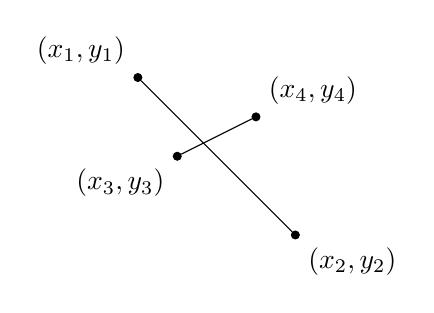
\begin{tikzpicture}        
        \node[circle, draw, fill, inner sep=1pt, label={135:$(x_1, y_1)$}] (a) at (0, 2) {};
        \node[circle, draw, fill, inner sep=1pt, label={-45:$(x_2, y_2)$}] (b) at (2, 0) {};
        \node[circle, draw, fill, inner sep=1pt, label={-135:$(x_3, y_3)$}] (c) at (0.5, 1) {};
        \node[circle, draw, fill, inner sep=1pt, label={45:$(x_4, y_4)$}] (d) at (1.5, 1.5) {};

        \draw (a) -- (b);
        \draw (c) -- (d);
    \end{tikzpicture}
\end{figure}
\noindent Then, the equations of the two lines are:
\begin{align*}
    (x_2 - x_1) (y - y_1) - (y_2 - y_1) (x - x_1) &= 0, \\
    (x_4 - x_3)(y - y_3) - (y_4 - y_3)(x - x_3) &= 0.
\end{align*}
We then find a point of intersection $(p, q)$ by solving the two equations simulatenously, if possible\sidefootnote{There are two cases when we won't be able to solve this system of equations easily- if the lines are parallel and have different $y$-offset, then they cannot intersect; if the two lines have the same $y$-offset, then they can intersect if the two segments overlap (i.e. $x_1 \leq x_3 \leq x_2$ or $x_1 \leq x_4 \leq x_2$, or vice versa).}. Finally, to check that the intersection of the two lines is within the line segments, we check that $x_1 \leq p \leq x_2$ and $x_3 \leq p \leq x_4$. The following figure illustrates why this is required:
\begin{figure}[H]
    \centering
    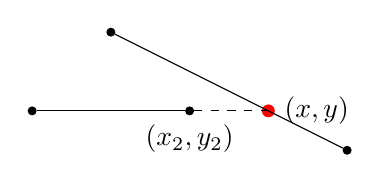
\begin{tikzpicture}
        \node[circle, draw, fill, inner sep=1pt] (a) at (0, 0) {};
        \node[circle, draw, fill, inner sep=1pt, label={-90:$(x_2, y_2)$}] (b) at (2, 0) {};
        \node[circle, draw, fill, inner sep=1pt] (c) at (1, 1) {};
        \node[circle, draw, fill, inner sep=1pt] (d) at (4, -0.5) {};
        \node[circle, draw, red, fill, inner sep=1.5pt, label={0:$(x, y)$}] at (3, 0) {};

        \draw (a) -- (b);
        \draw (c) -- (d);
        \draw[dashed] (b) -- (3, 0);
    \end{tikzpicture}
\end{figure}
\noindent Using the equation of the two lines, we will find that $(x, y)$ is a solution to the equation. However, we have $x > x_2$, so the intersection does not line on the line segment with $(x_2, y_2)$.

Although possible, this is not the most optimal way of solving the problem. The rearrangement to find the point of intersection involves division, which is susceptible to floating point errors. Moreover, we find the point of intersection even though we just need to find whether the line segments intersect- we are doing more work than required.

We will now look at a more efficient algorithm by breaking the problem down. If we have two line segments $p-q$ and $r-s$, then:
\begin{itemize}
    \item we first determine whether the two points $p$ and $q$ lie on different sides of the line $r-s$, and vice versa (\texttt{onOppositeSides}); and
    \item we then determine whether the smallest rectangles containing the lines $p-q$ and $r-s$ intersect (\texttt{boundingBox}).
\end{itemize}
The line segments intersect if and only if all the tests pass.

The algorithm \texttt{onOppositeSides} takes in two points $a$, $b$ and a line $-p1-p2-$, and determines whether $a$ and $b$ lie on opposite sides of the line. The equation of the line is given by
\[(l.p2.x - l.p1.x) (y - l.p1.y) - (l.p2.y - l.p1.y) (x - 1.p1.x) = 0.\]
When we substitute $(x, y)$ as the points $a$ and $b$, if the value at the LHS of the equation have different signs, then the two points lie on opposite sides. To see this, consider the following example:
\begin{figure}[H]
    \centering
    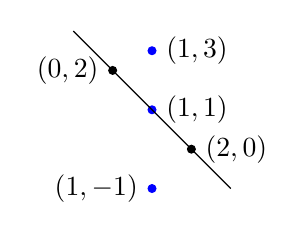
\begin{tikzpicture}
        \node[circle, draw, fill, inner sep=1pt, label={0:$(2, 0)$}] at (1.5, 0.5) {};
        \node[circle, draw, fill, inner sep=1pt, label={180:$(0, 2)$}] at (0.5, 1.5) {};
        \node[circle, draw, blue, fill, inner sep=1pt, label={0:$(1, 3)$}] at (1, 1.75) {};
        \node[circle, draw, blue, fill, inner sep=1pt, label={0:$(1, 1)$}] at (1, 1) {};
        \node[circle, draw, blue, fill, inner sep=1pt, label={180:$(1, -1)$}] at (1, 0) {};
        
        \draw (2, 0) -- (0, 2);
    \end{tikzpicture}
\end{figure}
\noindent Then, the equation of the line is $y + x - 2 = 0$. We can substitute the three blue points to the left hand side of the equation to get a value:
\begin{itemize}
    \item if $(x, y) = (1, 3)$, then $y + x - 2 = 2 > 0$;
    \item if $(x, y) = (1, 1)$, then $y + x - 2 = 0$;
    \item if $(x, y) = (1, -1)$, then $y + x - 2 = -2 < 0$.
\end{itemize}
In the figure above, all 3 pairs of points are considered to be on opposite sides- we consider $(1, 1)$ to be both above and below the line since it lies on the line. An easy way to check this is if the product of the two values to be non-negative. Note that we are meant to accept the case when both the lines are $(1, 1)$- this corresponds to the trivial line segment that intersects the line given at $(1, 1)$.

The algorithm \texttt{onOppositeSides} is given below.
\begin{lstlisting}[language=pseudocode]
bool onOppositeSides(Line line, Point a, Point b) {
    double v1 = (line.p2.x - line.p1.x) * (a.y - line.p1.y) - 
                (line.p2.y - line.p2.y) * (a.x - line.p1.x);
    double v2 = (line.p2.x - line.p1.x) * (b.y - line.p1.y) - 
                (line.p2.y - line.p2.y) * (b.x - line.p1.x);
    return v1 * v2 <= 0;
}
\end{lstlisting}


The condition \texttt{onOppositeSides} is not enough to check that the two line segments intersect. For example, consider the following line segments:
\begin{figure}[H]
    \centering
    \begin{tikzpicture}
        \node[circle, draw, fill, inner sep=1pt] (a) at (0, 2) {};
        \node[circle, draw, fill, inner sep=1pt] (b) at (0.5, 1.5) {};
        \node[circle, draw, fill, inner sep=1pt] (c) at (1, 1) {};
        \node[circle, draw, fill, inner sep=1pt] (d) at (2, 0) {};
        
        \draw (a) -- (b);
        \draw (c) -- (d);
    \end{tikzpicture}
\end{figure}
\noindent Since the two line segments are part of the same line, the result of \texttt{onOppositeSides} in both cases will be \texttt{true}. But, since the two line segments do not overlap, they do not intersect. For this reason, we require a third check- the bounding box.

The \emph{bounding box} of a line segment $p-q$ is the smallest rectangle that contains the line segment $p-q$ whose sides are parallel to the $x$ and the $y$-axes. For example, below is a line segment and its bounding box:
\begin{figure}[H]
    \centering
    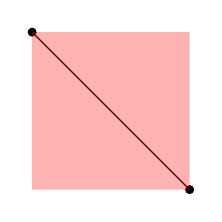
\begin{tikzpicture}
        \node[circle, draw, fill, inner sep=1pt] (a) at (2, 0) {};
        \node[circle, draw, fill, inner sep=1pt] (b) at (0, 2) {};

        \draw (a) -- (b);
        \fill[red, opacity=0.3] (2, 0) -- (2, 2) -- (0, 2) -- (0, 0) -- (2, 0);
    \end{tikzpicture}
\end{figure}
\noindent For two line segments to intersect, we require the bounding boxes to intersect. We illustrate this in the examples below:
\begin{figure}[H]
    \centering
    \begin{subfigure}{0.45\textwidth} 
        \centering
        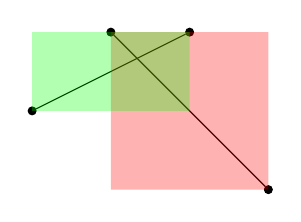
\begin{tikzpicture}
            \node[circle, draw, fill, inner sep=1pt] (a) at (2, 0) {};
            \node[circle, draw, fill, inner sep=1pt] (b) at (0, 2) {};
            \node[circle, draw, fill, inner sep=1pt] (c) at (1, 2) {};
            \node[circle, draw, fill, inner sep=1pt] (d) at (-1, 1) {};

            \draw (a) -- (b);
            \draw (c) -- (d);
            
            \fill[red, opacity=0.3] (2, 0) -- (2, 2) -- (0, 2) -- (0, 0) -- (2, 0);
            \fill[green, opacity=0.3] (1, 2) -- (-1, 2) -- (-1, 1) -- (1, 1) -- (1, 2);
        \end{tikzpicture}
    \end{subfigure}
    \hfill
    \begin{subfigure}{0.45\textwidth} 
        \centering
        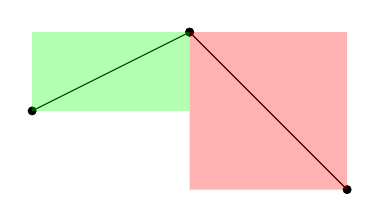
\begin{tikzpicture}
            \node[circle, draw, fill, inner sep=1pt] (a) at (2, 0) {};
            \node[circle, draw, fill, inner sep=1pt] (b) at (0, 2) {};
            \node[circle, draw, fill, inner sep=1pt] (c) at (0, 2) {};
            \node[circle, draw, fill, inner sep=1pt] (d) at (-2, 1) {};

            \draw (a) -- (b);
            \draw (c) -- (d);
            
            \fill[red, opacity=0.3] (2, 0) -- (2, 2) -- (0, 2) -- (0, 0) -- (2, 0);
            \fill[green, opacity=0.3] (0, 2) -- (-2, 2) -- (-2, 1) -- (0, 1) -- (0, 2);
        \end{tikzpicture}
    \end{subfigure}
\end{figure}
\noindent We see that when the two line segments intersect, their bounding boxes intersect. Also, if the bounding boxes do not intersect, then the two lines cannot intersect. Nonetheless, it is possible for two line segments to intersect and there to still not be an intersection- consider the following example.
\begin{figure}[H]
    \centering
    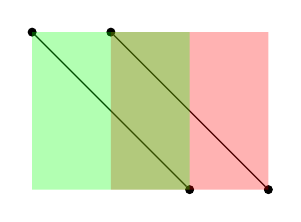
\begin{tikzpicture}
        \node[circle, draw, fill, inner sep=1pt] (a) at (2, 0) {};
        \node[circle, draw, fill, inner sep=1pt] (b) at (0, 2) {};
        \node[circle, draw, fill, inner sep=1pt] (c) at (1, 0) {};
        \node[circle, draw, fill, inner sep=1pt] (d) at (-1, 2) {};

        \draw (a) -- (b);
        \draw (c) -- (d);
        \fill[red, opacity=0.3] (2, 0) -- (2, 2) -- (0, 2) -- (0, 0) -- (2, 0);
        \fill[green, opacity=0.3] (1, 0) -- (1, 2) -- (-1, 2) -- (-1, 0) -- (1, 0);
    \end{tikzpicture}
\end{figure}
\noindent In this case, although the two lines do not intersect, their bounding boxes still intersect. The issue here is that in both line segments, the points are both on the same side of the other line segment.

Now, we consider how to define the \texttt{boundingBox} algorithm. The problem is essentially about when two rectangles intersect. So, consider the following two pairs of rectangles:
\begin{figure}[H]
    \centering
    \begin{subfigure}{0.4\textwidth} 
        \centering
        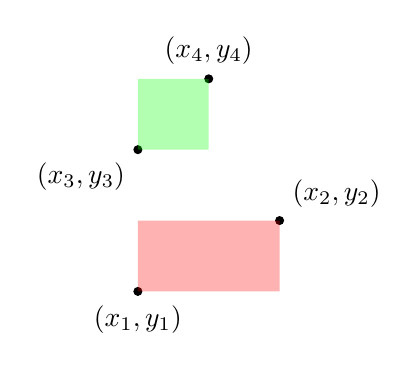
\begin{tikzpicture}[scale=0.9]
            \node[circle, draw, fill, inner sep=1pt, label={-90:$(x_1, y_1)$}] at (0, 0) {};
            \node[circle, draw, fill, inner sep=1pt, label={45:$(x_2, y_2)$}] at (2, 1) {};
            \node[circle, draw, fill, inner sep=1pt, label={-135:$(x_3, y_3)$}] at (0, 2) {};
            \node[circle, draw, fill, inner sep=1pt, label={90:$(x_4, y_4)$}] at (1, 3) {};

            \fill[red, opacity=0.3] (0, 0) -- (2, 0) -- (2, 1) -- (0, 1) -- (0, 0);
            \fill[green, opacity=0.3] (0, 2) -- (1, 2) -- (1, 3) -- (0, 3) -- (0, 2);
        \end{tikzpicture}
    \end{subfigure}
    \hfill
    \begin{subfigure}{0.55\textwidth} 
        \centering
        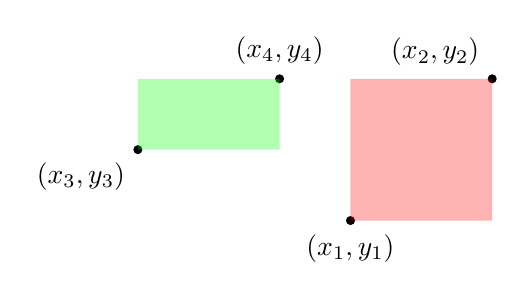
\begin{tikzpicture}[scale=0.9]
            \node[circle, draw, fill, inner sep=1pt, label={-90:$(x_1, y_1)$}] at (0, 0) {};
            \node[circle, draw, fill, inner sep=1pt, label={135:$(x_2, y_2)$}] at (2, 2) {};
            \node[circle, draw, fill, inner sep=1pt, label={-135:$(x_3, y_3)$}] at (-3, 1) {};
            \node[circle, draw, fill, inner sep=1pt, label={90:$(x_4, y_4)$}] at (-1, 2) {};

            \fill[red, opacity=0.3] (2, 0) -- (2, 2) -- (0, 2) -- (0, 0) -- (2, 0);
            \fill[green, opacity=0.3] (-1, 2) -- (-3, 2) -- (-3, 1) -- (-1, 1) -- (-1, 2);
        \end{tikzpicture}
    \end{subfigure}
\end{figure}
\noindent The rectangles on the left do not intersect since $y_3 > y_2$ and $x_3 > x_2$. On the other hand, the rectangles on the right do not intersect since $x_1 > x_4$ and $y_1 > y_4$. These give us four potential conditions required for rectangles to intersect- $x_3 \leq x_2, y_3 \leq y_2, x_1 \leq x_4, y_1 \leq y_4$. 

Assume now we fix one of the rectangles and consider what happens when the $x$-coordinates satisfy this condition:
\begin{figure}[H]
    \centering
    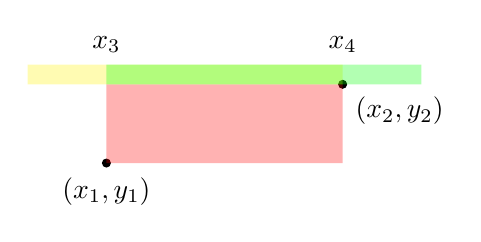
\begin{tikzpicture}
        \node[circle, draw, fill, inner sep=1pt, label={-90:$(x_1, y_1)$}] at (0, 0) {};
        \node[circle, draw, fill, inner sep=1pt, label={-45:$(x_2, y_2)$}] at (3, 1) {};

        \node at (0, 1.5) {$x_3$};
        \node at (3, 1.5) {$x_4$};

        \fill[red, opacity=0.3] (0, 0) -- (3, 0) -- (3, 1) -- (0, 1) -- (0, 0);
        \fill[yellow, opacity=0.3] (-1, 1) -- (3, 1) -- (3, 1.25) -- (-1, 1.25) -- (-1, 1);
        \fill[green, opacity=0.3] (0, 1) -- (4, 1) -- (4, 1.25) -- (0, 1.25) -- (0, 1);
    \end{tikzpicture}
\end{figure}
\noindent The value $x_3$ comes to the left of $x_2$, while the value $x_4$ comes to the right of $x_1$. In particular, $x_3$ can be at any point within the yellow region, and $x_4$ on the green region. This ensures that the two rectangles do intersect with respect to the $x$-coordinate. So, if we further require $y_3 \leq y_2$ and $y_1 \leq y_4$, the rectangles must intersect in both $x$- and $y$-coordinate, which means that they intersect in 2D. Therefore, these 4 conditions are sufficient. Hence, the algorithm \texttt{boundingBox} is the following.
\begin{lstlisting}[language=pseudocode]
bool boundingBox(LineSegment l1, LineSegment l2) {
    Rectangle r1 = new Rectangle(l1);
    Rectangle r2 = new Rectangle(l2);

    return  r2.bottomLeft.x <= r1.topRight.x &&
            r1.bottomLeft.x <= r2.topRight.x &&
            r2.bottomLeft.y <= r1.topRight.y &&
            r1.bottomLeft.y <= r2.topRight.y;
}
\end{lstlisting}

Putting this all together, we find that for line segments $p-q$ and $r-s$ intersect if and only if 
\begin{align*}
    \texttt{onOppositeSides(p, q, r-s)} &\land \texttt{onOppositeSides(r, s, p-q)} \\
    &\land \texttt{boundingBox(p-q, r-s)}.
\end{align*}
If two line segments intersect, then we know that for each of the line segment, the two points lie on opposite sides of the other one, and that their bounding boxes must intersect. So, this is a necessary condition for the line segments to intersect. Moreover, if two line segments do not intersect and their bounding boxes intersect, then one of them must be below the other, meaning that it is not on opposite sides- these conditions are sufficient as well.

Both the methods \texttt{onOppositeSides} and \texttt{boundingBox} are $O(1)$, so the intersection algorithm is also $O(1)$. Moreover, the algorithm does not involve division.

\newpage

\section{Simple Polygons and Convex Hulls}
In this section, we will look at constructing different polygons given a set of points. These polygons we construct will have various applications that we will consider later. First, we consider some further geometric objects:
\begin{itemize}
    \item a \emph{path} is a sequence of distinct points $p_1$ to $p_n$.
    \item a \emph{polygon} is a path where $p_1$ = $p_n$ (i.e. $p_1$ to $p_{n-1}$ are distinct, but $p_1 = p_n$);
    \item a \emph{simple polygon} is a polygon which does not intersect itself- it is characterised by partitioning the space into its interior and exterior;
    \item a \emph{convex polygon} is a simple polygon where for any two points $p$ and $q$ inside the polygon, the line segment $p-q$ is also inside it.
\end{itemize}
Below are some polygons that illustrate simple and convex polygons.
\begin{figure}[H]
    \centering
    \begin{subfigure}{0.3\textwidth}
        \centering
        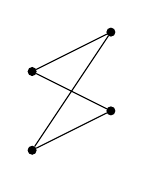
\begin{tikzpicture}
            \node[circle, draw, fill, inner sep=1pt] (a) at (0, 0) {};
            \node[circle, draw, fill, inner sep=1pt] (b) at (1, 0.5) {};
            \node[circle, draw, fill, inner sep=1pt] (c) at (0, 1) {};
            \node[circle, draw, fill, inner sep=1pt] (d) at (1, 1.5) {};

            \draw (a) -- (b) -- (c) -- (d) -- (a);
        \end{tikzpicture}
        \caption{A polygon that is not simple. The polygon crosses itself at the middle.}
    \end{subfigure}
    \hfill
    \begin{subfigure}{0.3\textwidth}
        \centering
        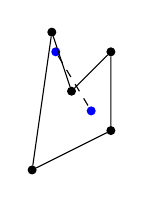
\begin{tikzpicture}
            \node[circle, draw, fill, inner sep=1pt] (a) at (0, 0) {};
            \node[circle, draw, fill, inner sep=1pt] (b) at (1, 0.5) {};
            \node[circle, draw, fill, inner sep=1pt] (c) at (1, 1.5) {};
            \node[circle, draw, fill, inner sep=1pt] (d) at (0.5, 1) {};
            \node[circle, draw, fill, inner sep=1pt] (e) at (0.25, 1.75) {};
            \node[circle, draw, blue, fill, inner sep=1pt] (f) at (0.3, 1.5) {};
            \node[circle, draw, blue, fill, inner sep=1pt] (g) at (0.75, 0.75) {};

            \draw (a) -- (b) -- (c) -- (d) -- (e) -- (a);
            \draw[dashed] (f) -- (g);
        \end{tikzpicture}
        \caption{A simple polygon that is not convex. The dashed line is not contained within the polygon.}
    \end{subfigure}
    \hfill
    \begin{subfigure}{0.3\textwidth}
        \centering
        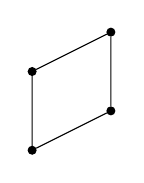
\begin{tikzpicture}
            \node[circle, draw, fill, inner sep=1pt] (a) at (0, 0) {};
            \node[circle, draw, fill, inner sep=1pt] (b) at (1, 0.5) {};
            \node[circle, draw, fill, inner sep=1pt] (c) at (0, 1) {};
            \node[circle, draw, fill, inner sep=1pt] (d) at (1, 1.5) {};

            \draw (a) -- (c) -- (d) -- (b) -- (a);
        \end{tikzpicture}
        \caption{A convex polygon.}
    \end{subfigure}
\end{figure}

\subsection{Simple Polygon}
We will now consider how to construct a simple polygon given a set of points. In the example above, we saw that it is not possible to construct a simple polygon by arbitrarily joining the set of points. So, we will need to reorder the points in the set so that the resulting set of points can be joined together pairwise to get a simple polygon.

To do so, we can choose a point on the plane as a pivot. Then, we scan the set of points in an anti-clockwise manner from the pivot to find the order in which we should construct the simple polygon. We illustrate this with an example.
\begin{figure}[H]
    \centering
    \begin{subfigure}{0.45\textwidth}
        \centering
        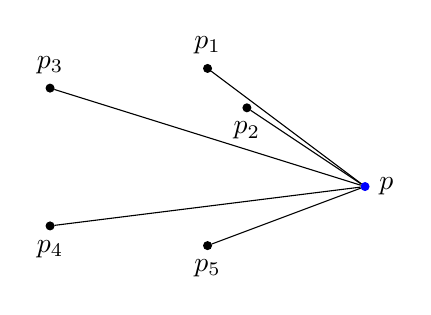
\begin{tikzpicture}
            \node[circle, draw, fill, blue, inner sep=1pt, label={0:$p$}] (p) at (4, 0.5) {};
            \node[circle, draw, fill, inner sep=1pt, label={90:$p_1$}] (p1) at (2, 2) {};
            \node[circle, draw, fill, inner sep=1pt, label={-90:$p_2$}] (p2) at (2.5, 1.5) {};
            \node[circle, draw, fill, inner sep=1pt, label={90:$p_3$}] (p3) at (0, 1.75) {};
            \node[circle, draw, fill, inner sep=1pt, label={-90:$p_4$}] (p4) at (0, 0) {};
            \node[circle, draw, fill, inner sep=1pt, label={-90:$p_5$}] (p5) at (2, -0.25) {};

            \draw (p) -- (p1);
            \draw (p) -- (p2);
            \draw (p) -- (p3);
            \draw (p) -- (p4);
            \draw (p) -- (p5);
        \end{tikzpicture}
    \end{subfigure}
    \hfill
    \begin{subfigure}{0.45\textwidth}
        \centering
        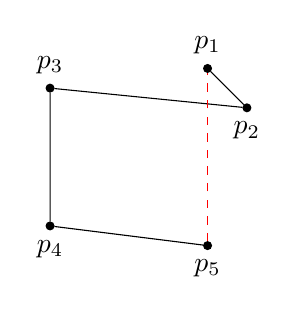
\begin{tikzpicture}
            \node[circle, draw, fill, inner sep=1pt, label={90:$p_1$}] (p1) at (2, 2) {};
            \node[circle, draw, fill, inner sep=1pt, label={-90:$p_2$}] (p2) at (2.5, 1.5) {};
            \node[circle, draw, fill, inner sep=1pt, label={90:$p_3$}] (p3) at (0, 1.75) {};
            \node[circle, draw, fill, inner sep=1pt, label={-90:$p_4$}] (p4) at (0, 0) {};
            \node[circle, draw, fill, inner sep=1pt, label={-90:$p_5$}] (p5) at (2, -0.25) {};

            \draw (p1) -- (p2) -- (p3) -- (p4) -- (p5);
            \draw[red, dashed] (p5) -- (p1);
        \end{tikzpicture}
    \end{subfigure}
\end{figure}
\noindent On the left, we use the pivot $p$ to scan and label the points going in an anti-clockwise fashion. That way, when we join the points $p_1 - p_2 - \dots - p_5$, we do not have any self-intersection. However, when we join $p_5$ and $p_1$, we do get a self-intersection. 

We can understand why there is a self-intersection using the figure below.
\begin{figure}[H]
    \centering
    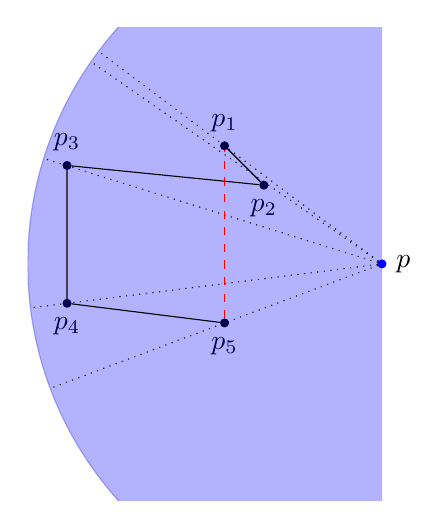
\begin{tikzpicture}
        \node[circle, draw, fill, blue, inner sep=1pt, label={0:$p$}] (p) at (4, 0.5) {};
        \node[circle, draw, fill, inner sep=1pt, label={90:$p_1$}] (p1) at (2, 2) {};
        \node[circle, draw, fill, inner sep=1pt, label={-90:$p_2$}] (p2) at (2.5, 1.5) {};
        \node[circle, draw, fill, inner sep=1pt, label={90:$p_3$}] (p3) at (0, 1.75) {};
        \node[circle, draw, fill, inner sep=1pt, label={-90:$p_4$}] (p4) at (0, 0) {};
        \node[circle, draw, fill, inner sep=1pt, label={-90:$p_5$}] (p5) at (2, -0.25) {};

        \begin{scope}
            \clip (4, -2.5) rectangle (-0.5, 3.5);
            \filldraw[blue, opacity=0.3] (p) circle (4.5);
        \end{scope}

        \draw[dotted] (p) -- (0.4, 3.2);
        \draw[dotted] (p) -- (0.30, 3.07);
        \draw[dotted] (p) -- (-0.30, 1.84);
        \draw[dotted] (p) -- (-0.47, -0.06);
        \draw[dotted] (p) -- (-0.21, -1.08);

        \draw (p1) -- (p2) -- (p3) -- (p4) -- (p5);
        \draw[red, dashed] (p5) -- (p1);
    \end{tikzpicture}
\end{figure}
\noindent The image represents a semi-circle centered at the pivot $p$. When we label each point, we partition the semi-circle into different sectors. And, when we connect two points, we go from one sector to another. If we exclude the last connection, there is only one line from one sector to another.

To avoid the intersection, we should choose the pivot as one of the points that we were given. The pivot is an extreme point- one way to choose the point would be to take the one with the highest $x$-coordinate (and lowest $y$-coordinate, if necessary). We first illustrate this with an example.
\begin{figure}[H]
    \centering
    \begin{subfigure}{0.45\textwidth}
        \centering
        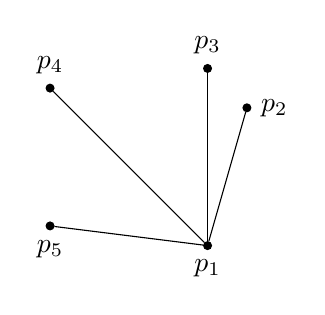
\begin{tikzpicture}
            \node[circle, draw, fill, inner sep=1pt, label={-90:$p_1$}] (p1) at (2, -0.25) {};
            \node[circle, draw, fill, inner sep=1pt, label={0:$p_2$}] (p2) at (2.5, 1.5) {};
            \node[circle, draw, fill, inner sep=1pt, label={90:$p_3$}] (p3) at (2, 2) {};
            \node[circle, draw, fill, inner sep=1pt, label={90:$p_4$}] (p4) at (0, 1.75) {};
            \node[circle, draw, fill, inner sep=1pt, label={-90:$p_5$}] (p5) at (0, 0) {};
            
            \draw (p1) -- (p2);
            \draw (p1) -- (p3);
            \draw (p1) -- (p4);
            \draw (p1) -- (p5);
        \end{tikzpicture}
    \end{subfigure}
    \hfill
    \begin{subfigure}{0.45\textwidth}
        \centering
        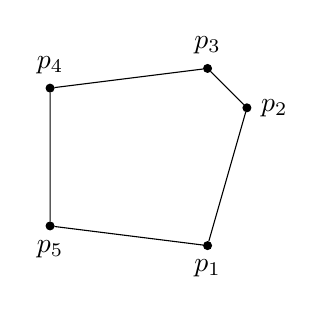
\begin{tikzpicture}
            \node[circle, draw, fill, inner sep=1pt, label={-90:$p_1$}] (p1) at (2, -0.25) {};
            \node[circle, draw, fill, inner sep=1pt, label={0:$p_2$}] (p2) at (2.5, 1.5) {};
            \node[circle, draw, fill, inner sep=1pt, label={90:$p_3$}] (p3) at (2, 2) {};
            \node[circle, draw, fill, inner sep=1pt, label={90:$p_4$}] (p4) at (0, 1.75) {};
            \node[circle, draw, fill, inner sep=1pt, label={-90:$p_5$}] (p5) at (0, 0) {};
            
            \draw (p1) -- (p2) -- (p3) -- (p4) -- (p5) -- (p1);
        \end{tikzpicture}
    \end{subfigure}
\end{figure}
\noindent Here, the pivot was $p_1$. Using this pivot, we labelled the other points depending on when we encountered it with respect to the pivot, turning anti-clockwise. As we can see, this does not lead to a self-intersection at the end. 

We will now use a similar diagram to above to show that this method always works.
\begin{figure}[H]
    \centering
    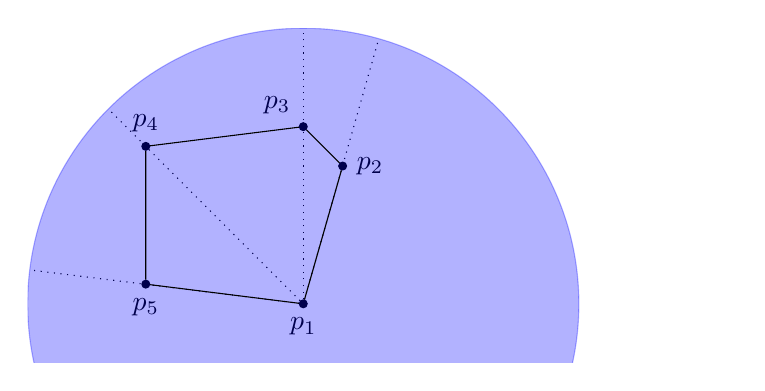
\begin{tikzpicture}
        \node[circle, draw, fill, inner sep=1pt, label={-90:$p_1$}] (p1) at (2, -0.25) {};
        \node[circle, draw, fill, inner sep=1pt, label={0:$p_2$}] (p2) at (2.5, 1.5) {};
        \node[circle, draw, fill, inner sep=1pt, label={135:$p_3$}] (p3) at (2, 2) {};
        \node[circle, draw, fill, inner sep=1pt, label={90:$p_4$}] (p4) at (0, 1.75) {};
        \node[circle, draw, fill, inner sep=1pt, label={-90:$p_5$}] (p5) at (0, 0) {};
        
        \draw[dotted] (p1) -- (2.96, 3.12);
        \draw[dotted] (p1) -- (2, 3.25);
        \draw[dotted] (p1) -- (-0.47, 2.22);
        \draw[dotted] (p1) -- (-1.47, 0.18);

        \begin{scope}
            \clip (-1.5, -1) rectangle (7.5, 3.25);
            \filldraw[blue, opacity=0.3] (p1) circle (3.5);
        \end{scope}
        
        \draw (p1) -- (p2) -- (p3) -- (p4) -- (p5) -- (p1);
    \end{tikzpicture}
\end{figure}
\noindent Like before, we do not expect there to be an intersect going from a point to a non-final point. Moreover, at the end, we are traveling along the radius- this ensures that we do not move to another sector and get a self-intersection.

Next, we consider the algorithm. To label the points, we sort them with respect to the angle it makes with the pivot- the smaller the angle, the earlier it is placed. The following is the algorithm:
\begin{lstlisting}[language=pseudocode]
void simplePolygon(List<Point> points) {
    // find the pivot
    int i  = 0;
    Point pivot = points[0];
    for (int j = 1; j < points.length; j++) {
        // Change the pivot if this point has x-coordinate bigger 
        // or if this point has the same x-coordinate, and the 
        // y-coordinate is smaller.
        if (pivot.x < points[j].x || 
            (pivot.x == points[j].x && pivot.y < points[j].y)) {
            pivot = points[j];
            i = j;
        }
    }
    
    // move the pivot to the start
    points[i] = points[0];
    points[0] = pivot;
    
    Map<Point, double> angles = {};
    Map<Point, double> distances = {};
    
    // sort the points wrt angle it makes with the pivot
    points.sort((p1, p2) {
        double angle1 = angles[p1] ?? 
                        atan2(pivot.x-p1.x, pivot.y-p1.y);
        angles[p1] = angle1;
    
        double angle2 = angles[p2] ?? 
                        atan2(pivot.x - p2.x, pivot.y - p2.y);
        angles[p2] = angle2;
    
        return angle1.compareTo(angle2);
    });
}
\end{lstlisting}
The function \texttt{atan2} takes in the numerator and the denominator of the \texttt{arctan} function as two different arguments and gives the right \texttt{arctan} value, e.g. if the denominator is 0 or if the angle is greater than $\pi$.

We now consider the complexity of the algorithm- if there are $n$ points, then the loop to compute angles is $O(n)$, and the sorting is $O(n \log n)$. Therefore, the total complexity is $O(n \log n)$. So, this is a very efficient algorithm. It does use the \texttt{arctan} function, which is considered expensive. Moreover, there is no reason to explicitly compute the angles. We will now illustrate how to label the points without explicitly compute the arctangent value. So, consider the previous pivot labelling:
\begin{figure}[H]
    \centering
    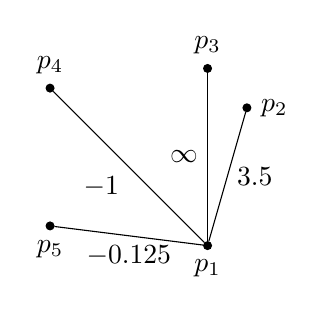
\begin{tikzpicture}
        \node[circle, draw, fill, inner sep=1pt, label={-90:$p_1$}] (p1) at (2, -0.25) {};
        \node[circle, draw, fill, inner sep=1pt, label={0:$p_2$}] (p2) at (2.5, 1.5) {};
        \node[circle, draw, fill, inner sep=1pt, label={90:$p_3$}] (p3) at (2, 2) {};
        \node[circle, draw, fill, inner sep=1pt, label={90:$p_4$}] (p4) at (0, 1.75) {};
        \node[circle, draw, fill, inner sep=1pt, label={-90:$p_5$}] (p5) at (0, 0) {};
        
        \draw (p1) -- node[right] {$3.5$} (p2);
        \draw (p1) -- node[left] {$\infty$} (p3);
        \draw (p1) -- node[below left] {$-1$} (p4);
        \draw (p1) -- node[below] {$-0.125$} (p5);
    \end{tikzpicture}
\end{figure}
\noindent The labelled numbers are the gradients of the line going between $p_1$ and $p_i$ for $2 \leq i \leq 5$. So, given two gradients $m_1$ and $m_2$, we compare them as follows:
\begin{itemize}
    \item if $m_1$ and $m_2$ have different signs, then the positive one comes first;
    \item if $m_1$ and $m_2$ have the same sign, then the smaller one comes first.
\end{itemize}
Using this pattern, we can sort the values by just comparing the gradients. This can be done without any division too, i.e. if we have
\[m_1 = \frac{dy_1}{dx_1}, \qquad m_2 = \frac{dy_2}{dx_2},\]
then we can cross multiply to find out whether $m_1$ should come before $m_2$- we need to pay attention to the sign of the values being multiplied to return the correct result.

Although the algorithm works in most cases, it does not consider the following exceptional cases:
\begin{itemize}
    \item If all the points are collinear with respect to the pivot, then there is no enclosing polygon.
    \item If points are collinear with respect to the pivot, they can be sorted in any order. However, we would require them to be sorted in the `right' order. For instance, consider the following example:
    \begin{figure}[H]
        \centering
        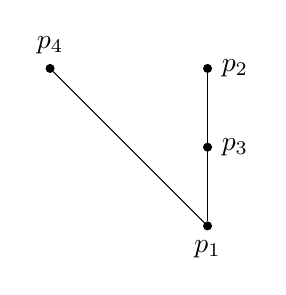
\begin{tikzpicture}
            \node[circle, draw, fill, inner sep=1pt, label={-90:$p_1$}] (p1) at (2, 0) {};
            \node[circle, draw, fill, inner sep=1pt, label={0:$p_2$}] (p2) at (2, 2) {};
            \node[circle, draw, fill, inner sep=1pt, label={0:$p_3$}] (p3) at (2, 1) {};
            \node[circle, draw, fill, inner sep=1pt, label={90:$p_4$}] (p4) at (0, 2) {};
            
            \draw (p1) -- (p2);
            \draw (p1) -- (p4);
        \end{tikzpicture}
    \end{figure}
    \noindent Here, the pivot is $p_1$. Since $p_2$ and $p_3$ make the same angle with the pivot, we would need to choose the right order- the current ordering does not give us a simple polygon since $p_3$ should be the top right point. We mitigate this by further sorting the points by the distance it makes with the pivot.
    \item If the final points are collinear to the pivot, then sorting them by increasing distance from the pivot does not work. For instance, consider the following example:
    \begin{figure}[H]
        \centering
        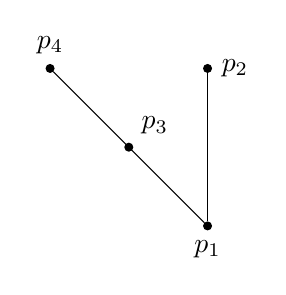
\begin{tikzpicture}
            \node[circle, draw, fill, inner sep=1pt, label={-90:$p_1$}] (p1) at (2, 0) {};
            \node[circle, draw, fill, inner sep=1pt, label={0:$p_2$}] (p2) at (2, 2) {};
            \node[circle, draw, fill, inner sep=1pt, label={90:$p_4$}] (p4) at (0, 2) {};
            \node[circle, draw, fill, inner sep=1pt, label={45:$p_3$}] (p3) at (1, 1) {};
            
            \draw (p1) -- (p2);
            \draw (p1) -- (p4);
        \end{tikzpicture}
    \end{figure}
    \noindent Here, the pivot is $p_1$. Since $p_3$ and $p_4$ make the same angle with the pivot, we would sort $p_3$ and $p_4$ in the order given above by the observation we made in the previous point. However, this does not work when the point is getting connected to the pivot. In that case, we would need to reverse these points, i.e. sort them with respect to the largest distance with the pivot, not the smallest.
\end{itemize}

\subsection{Convex Hull}
Now, we will consider the convex hull problem. For a set of points on the plane, the convex hull is the smallest convex polygon that contains all the points. We measure the size of the polygon by its perimeter. So, we expect some of the points to lie on the boundary of this polygon. It is possible that not all of them lie on the boundary, as shown in the figure below.
\begin{figure}[H]
    \centering
    \begin{subfigure}{0.3\textwidth}
        \centering
        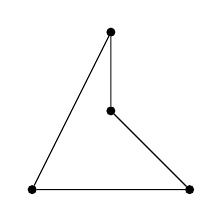
\begin{tikzpicture}
            \node[circle, draw, fill, inner sep=1pt] (a) at (0, 0) {};
            \node[circle, draw, fill, inner sep=1pt] (b) at (2, 0) {};
            \node[circle, draw, fill, inner sep=1pt] (c) at (1, 1) {};
            \node[circle, draw, fill, inner sep=1pt] (d) at (1, 2) {};

            \draw (a) -- (b) -- (c) -- (d) -- (a);
        \end{tikzpicture}
    \end{subfigure}
    \hfill
    \begin{subfigure}{0.3\textwidth}
        \centering
        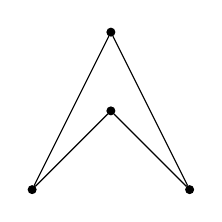
\begin{tikzpicture}
            \node[circle, draw, fill, inner sep=1pt] (a) at (0, 0) {};
            \node[circle, draw, fill, inner sep=1pt] (b) at (2, 0) {};
            \node[circle, draw, fill, inner sep=1pt] (c) at (1, 1) {};
            \node[circle, draw, fill, inner sep=1pt] (d) at (1, 2) {};

            \draw (a) -- (c) -- (b) -- (d) -- (a);
        \end{tikzpicture}
    \end{subfigure}
    \hfill
    \begin{subfigure}{0.3\textwidth}
        \centering
        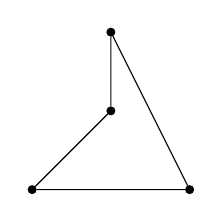
\begin{tikzpicture}
            \node[circle, draw, fill, inner sep=1pt] (a) at (0, 0) {};
            \node[circle, draw, fill, inner sep=1pt] (b) at (2, 0) {};
            \node[circle, draw, fill, inner sep=1pt] (c) at (1, 1) {};
            \node[circle, draw, fill, inner sep=1pt] (d) at (1, 2) {};

            \draw (a) -- (b) -- (d) -- (c) -- (a);
        \end{tikzpicture}
    \end{subfigure}
\end{figure}
\noindent In the figure above, we have 3 simple polygons from the same set of points. These are the only simple polygons containing all the points. Clearly, none of these are convex polygons. In fact, the convex hull of these 4 points is the following:
\begin{figure}[H]
    \centering
    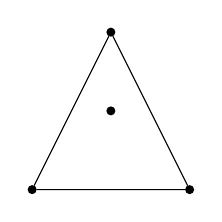
\begin{tikzpicture}
        \node[circle, draw, fill, inner sep=1pt] (a) at (0, 0) {};
        \node[circle, draw, fill, inner sep=1pt] (b) at (2, 0) {};
        \node[circle, draw, fill, inner sep=1pt] (c) at (1, 1) {};
        \node[circle, draw, fill, inner sep=1pt] (d) at (1, 2) {};

        \draw (a) -- (b) -- (d) -- (a);
    \end{tikzpicture}
\end{figure}

In a given set of points, the point that has the smallest or the largest $x$/$y$-coordinate will always lie on the convex hull. This implies that the choice of pivot from the simple polygon algorithm above will still work in this case.

% Also, the two points in the set with the largest distance also lie on the convex hull. 

The algorithm for constructing the convex hull is the Graham Scan algorithm. It starts by running the simple polygon algorithm to sort the set of points with respect to the angle they make with the pivot. We then add these points in order to the convex hull, and remove any points as we realise that shouldn't lie on it. One way of finding out whether a point should be included is to:
\begin{itemize}
    \item choose the pivot to be the point with the largest $x$-coordinate (and smallest $y$-coordinate); and
    \item choose to keep a point $p_i$ if, when adding the next point $p_{i+1}$, the triplet $(p_{i+1}, p_i, p_{i-1})$, the anti-clockwise angle between the two lines is less than $\pi$.
\end{itemize}

We illustrate the procedure with an example. Consider the following set of points.
\begin{figure}[H]
    \centering
    \begin{tikzpicture}
        \node[circle, draw, fill, inner sep=1pt, label={0:$p_1$}] (p1) at (3, 0) {};
        \node[circle, draw, fill, inner sep=1pt, label={0:$p_2$}] (p2) at (3.75, 1.5) {};
        \node[circle, draw, fill, inner sep=1pt, label={0:$p_3$}] (p3) at (2.25, 2.25) {};
        \node[circle, draw, fill, inner sep=1pt, label={-135:$p_4$}] (p4) at (2.25, 1.25) {};
        \node[circle, draw, fill, inner sep=1pt, label={0:$p_5$}] (p5) at (1.5, 1.5) {};
        \node[circle, draw, fill, inner sep=1pt, label={180:$p_6$}] (p6) at (0, 0.75) {};
    \end{tikzpicture}
\end{figure}
\noindent We have already applied the simple polygon algorithm to label the points with respect to the pivot $p_1$. We first connect the first three points- it is guaranteed that the angle between $-p_1-p_2-$ and $-p_2-p_3$ is less than $\pi$, since the angles have been sorted in increasing order with respect to $p_1$. 
\begin{figure}[H]
    \centering
    \begin{tikzpicture}
        \node[circle, draw, fill, inner sep=1pt, label={0:$p_1$}] (p1) at (3, 0) {};
        \node[circle, draw, fill, inner sep=1pt, label={0:$p_2$}] (p2) at (3.75, 1.5) {};
        \node[circle, draw, fill, inner sep=1pt, label={0:$p_3$}] (p3) at (2.25, 2.25) {};
        \node[circle, draw, fill, inner sep=1pt, label={-135:$p_4$}] (p4) at (2.25, 1.25) {};
        \node[circle, draw, fill, inner sep=1pt, label={0:$p_5$}] (p5) at (1.5, 1.5) {};
        \node[circle, draw, fill, inner sep=1pt, label={180:$p_6$}] (p6) at (0, 0.75) {};

        \draw (p1) -- (p2) -- (p3);
        \draw[blue] (p3) -- (p4);
        \draw[dashed] (p3) -- (1, 2.875);
        \draw[->] (2, 2.375) arc (135:275:0.25);
    \end{tikzpicture}
\end{figure}
\noindent The next point to add is $p_4$. The angle between the two lines $-p_2-p_3-$ and $-p_3-p_4-$ is less than $\pi$, so we do not remove $p_3$.
\begin{figure}[H]
    \centering
    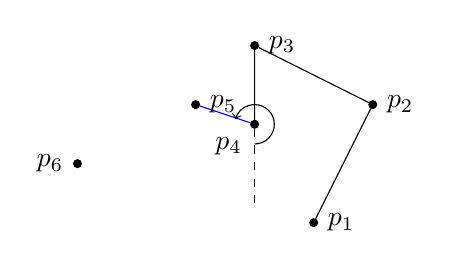
\begin{tikzpicture}
        \node[circle, draw, fill, inner sep=1pt, label={0:$p_1$}] (p1) at (3, 0) {};
        \node[circle, draw, fill, inner sep=1pt, label={0:$p_2$}] (p2) at (3.75, 1.5) {};
        \node[circle, draw, fill, inner sep=1pt, label={0:$p_3$}] (p3) at (2.25, 2.25) {};
        \node[circle, draw, fill, inner sep=1pt, label={-135:$p_4$}] (p4) at (2.25, 1.25) {};
        \node[circle, draw, fill, inner sep=1pt, label={0:$p_5$}] (p5) at (1.5, 1.5) {};
        \node[circle, draw, fill, inner sep=1pt, label={180:$p_6$}] (p6) at (0, 0.75) {};

        \draw (p1) -- (p2) -- (p3) -- (p4);
        \draw[blue] (p4) -- (p5);
        \draw[dashed] (p4) -- (2.25, 0.25);
        \draw[->] (2.25, 1) arc (-90:165:0.25);
    \end{tikzpicture}
\end{figure}
\noindent The next point to add is $p_5$. However, the corresponding angle is clearly bigger than $\pi$, so we will first need to discard $p_4$.
\begin{figure}[H]
    \centering
    \begin{tikzpicture}
        \node[circle, draw, fill, inner sep=1pt, label={0:$p_1$}] (p1) at (3, 0) {};
        \node[circle, draw, fill, inner sep=1pt, label={0:$p_2$}] (p2) at (3.75, 1.5) {};
        \node[circle, draw, fill, inner sep=1pt, label={0:$p_3$}] (p3) at (2.25, 2.25) {};
        \node[circle, draw, fill, inner sep=1pt, label={-135:$p_4$}] (p4) at (2.25, 1.25) {};
        \node[circle, draw, fill, inner sep=1pt, label={0:$p_5$}] (p5) at (1.5, 1.5) {};
        \node[circle, draw, fill, inner sep=1pt, label={180:$p_6$}] (p6) at (0, 0.75) {};

        \draw (p1) -- (p2) -- (p3);
        \draw[blue] (p3) -- (p5);
        \draw[dashed] (p3) -- (1, 2.875);
        \draw[->] (2, 2.375) arc (135:240:0.25);
    \end{tikzpicture}
\end{figure}
\noindent Now, the angle is less than $\pi$. So, we add $p_5$ to the convex hull.
\begin{figure}[H]
    \centering
    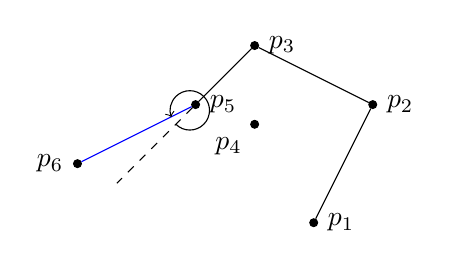
\begin{tikzpicture}
        \node[circle, draw, fill, inner sep=1pt, label={0:$p_1$}] (p1) at (3, 0) {};
        \node[circle, draw, fill, inner sep=1pt, label={0:$p_2$}] (p2) at (3.75, 1.5) {};
        \node[circle, draw, fill, inner sep=1pt, label={0:$p_3$}] (p3) at (2.25, 2.25) {};
        \node[circle, draw, fill, inner sep=1pt, label={-135:$p_4$}] (p4) at (2.25, 1.25) {};
        \node[circle, draw, fill, inner sep=1pt, label={0:$p_5$}] (p5) at (1.5, 1.5) {};
        \node[circle, draw, fill, inner sep=1pt, label={180:$p_6$}] (p6) at (0, 0.75) {};

        \draw (p1) -- (p2) -- (p3) -- (p5);
        \draw[blue] (p5) -- (p6);
        \draw[dashed] (p5) -- (0.5, 0.5);
        \draw[->] (1.25, 1.25) arc (-135:200:0.25);
    \end{tikzpicture}
\end{figure}
\noindent This angle is also more than $\pi$, so we have to discard $p_5$ too.
\begin{figure}[H]
    \centering
    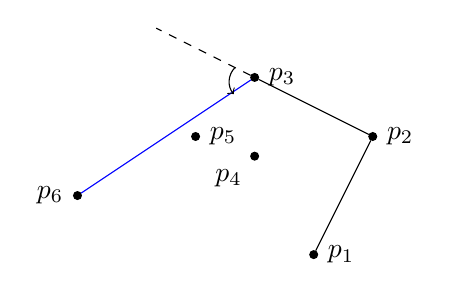
\begin{tikzpicture}
        \node[circle, draw, fill, inner sep=1pt, label={0:$p_1$}] (p1) at (3, 0) {};
        \node[circle, draw, fill, inner sep=1pt, label={0:$p_2$}] (p2) at (3.75, 1.5) {};
        \node[circle, draw, fill, inner sep=1pt, label={0:$p_3$}] (p3) at (2.25, 2.25) {};
        \node[circle, draw, fill, inner sep=1pt, label={-135:$p_4$}] (p4) at (2.25, 1.25) {};
        \node[circle, draw, fill, inner sep=1pt, label={0:$p_5$}] (p5) at (1.5, 1.5) {};
        \node[circle, draw, fill, inner sep=1pt, label={180:$p_6$}] (p6) at (0, 0.75) {};

        \draw (p1) -- (p2) -- (p3);
        \draw[blue] (p3) -- (p6);
        \draw[dashed] (p3) -- (1, 2.875);
        \draw[->] (2, 2.375) arc (135:220:0.25);
    \end{tikzpicture}
\end{figure}
\noindent The angle the lines $-p_2-p_3-$ and $-p_3-p_6-$ make is less than $\pi$, so $p_6$ gets added to the convex hull. Since it is the last point, we have constructed the convex hull:
\begin{figure}[H]
    \centering
    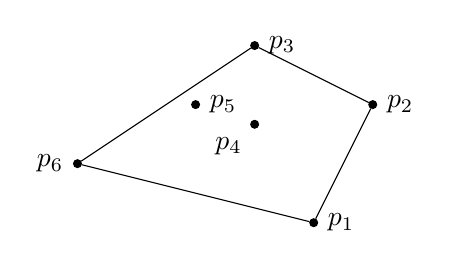
\begin{tikzpicture}
        \node[circle, draw, fill, inner sep=1pt, label={0:$p_1$}] (p1) at (3, 0) {};
        \node[circle, draw, fill, inner sep=1pt, label={0:$p_2$}] (p2) at (3.75, 1.5) {};
        \node[circle, draw, fill, inner sep=1pt, label={0:$p_3$}] (p3) at (2.25, 2.25) {};
        \node[circle, draw, fill, inner sep=1pt, label={-135:$p_4$}] (p4) at (2.25, 1.25) {};
        \node[circle, draw, fill, inner sep=1pt, label={0:$p_5$}] (p5) at (1.5, 1.5) {};
        \node[circle, draw, fill, inner sep=1pt, label={180:$p_6$}] (p6) at (0, 0.75) {};

        \draw (p1) -- (p2) -- (p3) -- (p6) -- (p1);
    \end{tikzpicture}
\end{figure}
\noindent We are guaranteed to make the right angle when we connect the last point with the pivot, as long as the pivot belongs to the convex hull.

The algorithm for the Graham Scan is given below.
% TODO: Add algorithm

Now, we consider the complexity of the algorithm. The algorithm uses simple polygon construction, which has $O(n \log n)$ complexity. We can check whether the turn is anti-clockwise in $O(1)$ time. Now, the while loop within the for loop could imply that the complexity is $O(n^2)$. However, since a point is eliminated at most once from the list, the complexity of the entire loop is $O(n)$. Hence, the algorithm has complexity $O(n \log n)$.

Next, we will consider some applications of the convex hull algorithm. A basic usage might be for a robot to avoid some obstacles, while taking the shortest path. That is, the robot is at position $A$, wants to get to position $B$, and there are some obstacles in the middle. Then, we consider the set of points containing the obstacles and the positions $A$ and $B$. We construct a convex hull for this set of points. The shortest path avoiding the obstacles will then be either the clockwise or the anti-clockwise path from $A$ to $B$.

Another application is to compute the furthest pair of points in a set of points. A naive method would check each pair of points- that is $O(n^2)$. However, we can use the convex hull and compute the furthest pair of points in $O(n \log n)$ time- this is because the convex hull contains the pair of points that are furthest from each other.
% TODO: Illustrate this
\begin{figure}[H]
    \centering
    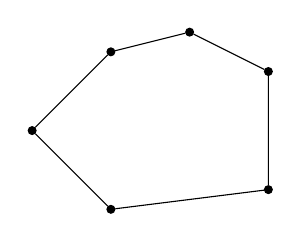
\begin{tikzpicture}
        \node[circle, draw, fill, inner sep=1pt] (p1) at (0, 0) {};
        \node[circle, draw, fill, inner sep=1pt] (p2) at (1, 1) {};
        \node[circle, draw, fill, inner sep=1pt] (p3) at (2, 1.25) {};
        \node[circle, draw, fill, inner sep=1pt] (p4) at (3, 0.75) {};
        \node[circle, draw, fill, inner sep=1pt] (p5) at (3, -0.75) {};
        \node[circle, draw, fill, inner sep=1pt] (p6) at (1, -1) {};

        \draw (p1) -- (p2) -- (p3) -- (p4) -- (p5) -- (p6) -- (p1);
    \end{tikzpicture}
\end{figure}
\noindent We first select 2 points- one that has a maximum $x$-coordinate, and a minimum $y$-coordinate.
\begin{figure}[H]
    \centering
    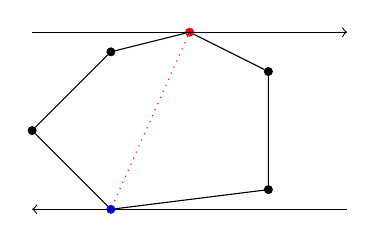
\begin{tikzpicture}
        \node[circle, draw, fill, inner sep=1pt] (p1) at (0, 0) {};
        \node[circle, draw, fill, inner sep=1pt] (p2) at (1, 1) {};
        \node[circle, draw, fill, red, inner sep=1pt] (p3) at (2, 1.25) {};
        \node[circle, draw, fill, inner sep=1pt] (p4) at (3, 0.75) {};
        \node[circle, draw, fill, inner sep=1pt] (p5) at (3, -0.75) {};
        \node[circle, draw, fill, blue, inner sep=1pt] (p6) at (1, -1) {};

        \draw (p1) -- (p2) -- (p3) -- (p4) -- (p5) -- (p6) -- (p1);

        \draw[->] (0, 1.25) -- (4, 1.25);
        \draw[<-] (0, -1) -- (4, -1);

        \draw[dotted, red] (p3) -- (p6);
    \end{tikzpicture}
\end{figure}
\noindent We keep track of the distances between any two points we encounter. We rotate in clockwise direction, until we hit another point.
\begin{figure}[H]
    \centering
    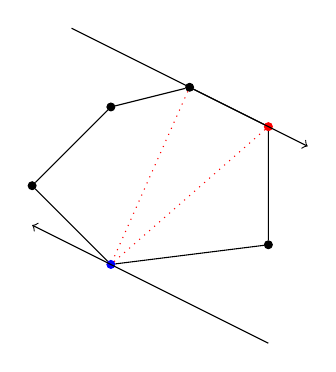
\begin{tikzpicture}
        \node[circle, draw, fill, inner sep=1pt] (p1) at (0, 0) {};
        \node[circle, draw, fill, inner sep=1pt] (p2) at (1, 1) {};
        \node[circle, draw, fill, inner sep=1pt] (p3) at (2, 1.25) {};
        \node[circle, draw, fill, red, inner sep=1pt] (p4) at (3, 0.75) {};
        \node[circle, draw, fill, inner sep=1pt] (p5) at (3, -0.75) {};
        \node[circle, draw, fill, blue, inner sep=1pt] (p6) at (1, -1) {};

        \draw (p1) -- (p2) -- (p3) -- (p4) -- (p5) -- (p6) -- (p1);
        
        \draw[->] (0.5, 2) -- (3.5, 0.5);
        \draw[<-] (0, -0.5) -- (3, -2);

        \draw[dotted, red] (p3) -- (p6);
        \draw[dotted, red] (p4) -- (p6);
    \end{tikzpicture}
\end{figure}
\noindent We continue this until the two lines have flipped.
\begin{figure}[H]
    \centering
    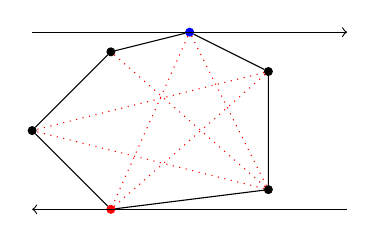
\begin{tikzpicture}
        \node[circle, draw, fill, inner sep=1pt] (p1) at (0, 0) {};
        \node[circle, draw, fill, inner sep=1pt] (p2) at (1, 1) {};
        \node[circle, draw, fill, blue, inner sep=1pt] (p3) at (2, 1.25) {};
        \node[circle, draw, fill, inner sep=1pt] (p4) at (3, 0.75) {};
        \node[circle, draw, fill, inner sep=1pt] (p5) at (3, -0.75) {};
        \node[circle, draw, fill, red, inner sep=1pt] (p6) at (1, -1) {};

        \draw (p1) -- (p2) -- (p3) -- (p4) -- (p5) -- (p6) -- (p1);
        
        % \draw[->] (0.5, 2) -- (3.5, 0.5);
        % \draw[<-] (0, -0.5) -- (3, -2);

        \draw[dotted, red] (p3) -- (p6);
        \draw[dotted, red] (p3) -- (p5);
        \draw[dotted, red] (p4) -- (p6);
        \draw[dotted, red] (p4) -- (p1);
        \draw[dotted, red] (p5) -- (p1);
        \draw[dotted, red] (p5) -- (p2);

        \draw[->] (0, 1.25) -- (4, 1.25);
        \draw[<-] (0, -1) -- (4, -1);
    \end{tikzpicture}
\end{figure}
\noindent Then, we choose the pair such that the distance is the longest- this is the longest distance of the entire set of points, not just the convex hull. This algorithm is called the rolling calipers.


\end{document}
